\newpage
\chapter{Isomap}
\section{Eindimensionales Signal}
\begin{figure}[h]
	\centering
	\subfloat[Caption for sub-figure1]{
		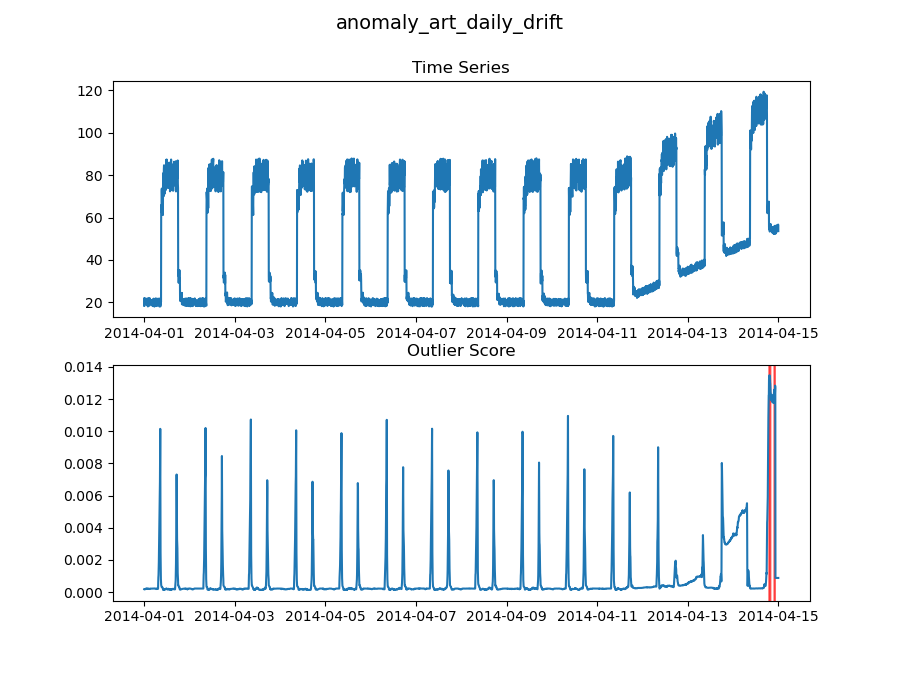
\includegraphics[width=0.5\textwidth]{fig/resultsIsoMap/anomaly_art_daily_drift}}
	\subfloat[Caption for sub-figure1]{
		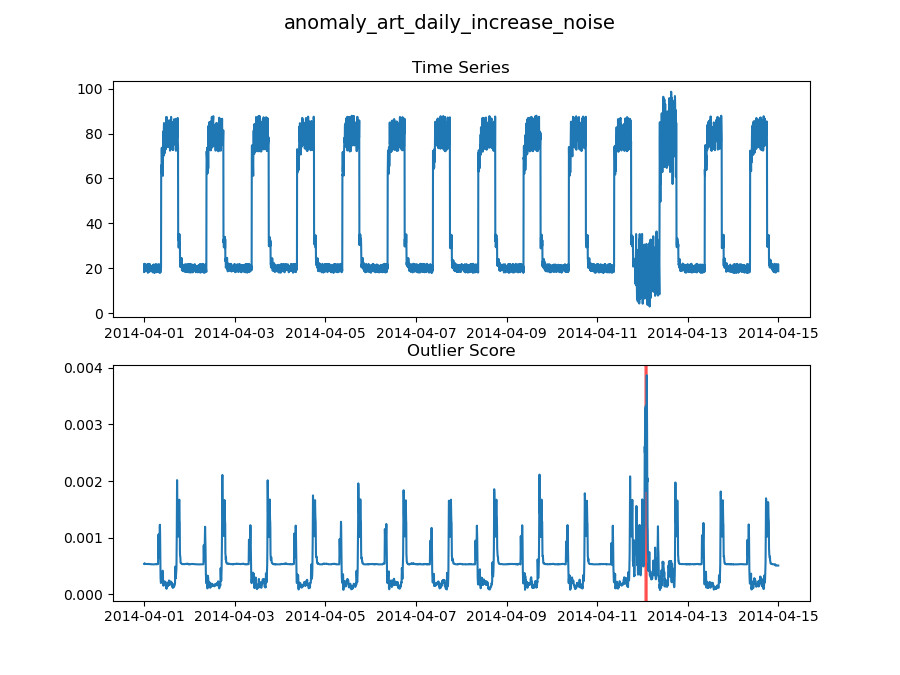
\includegraphics[width=0.5\textwidth]{fig/resultsIsoMap/anomaly_art_daily_increase_noise}}
	\qquad
	\subfloat[Caption for sub-figure1]{
		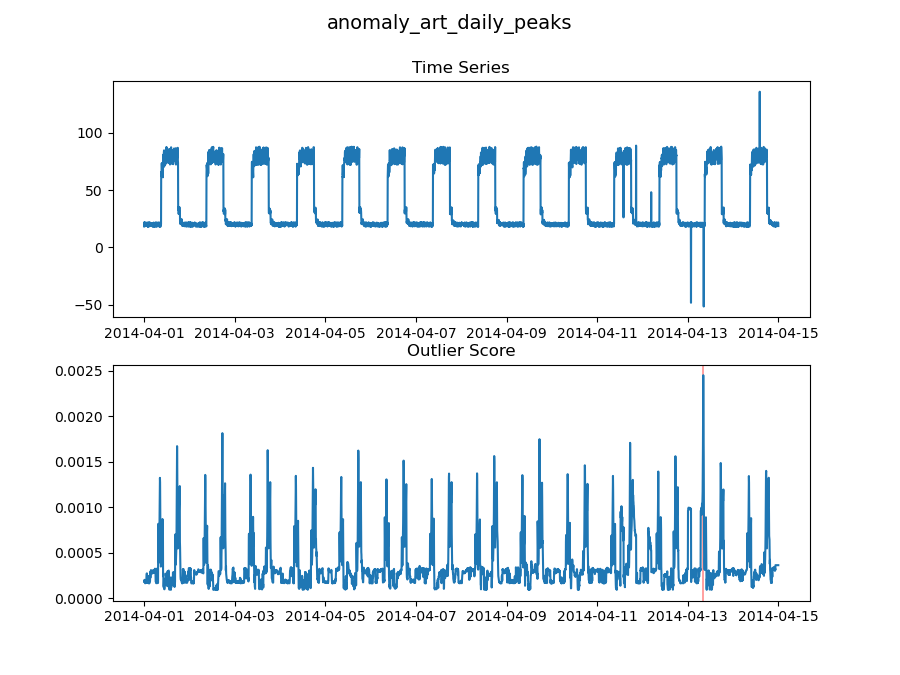
\includegraphics[width=0.5\textwidth]{fig/resultsIsoMap/anomaly_art_daily_peaks}}
	\subfloat[Caption for sub-figure1]{
		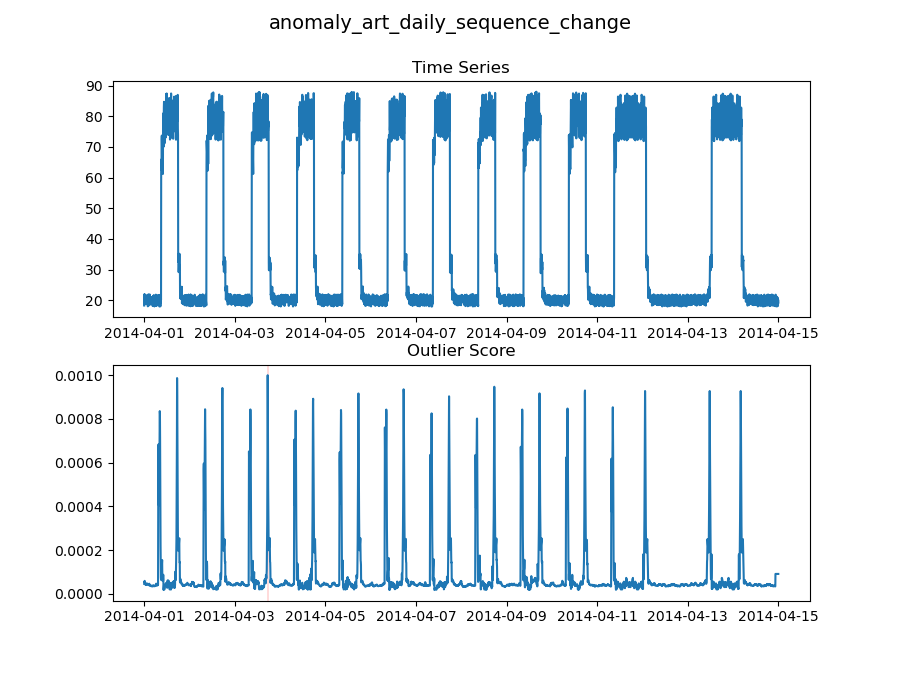
\includegraphics[width=0.5\textwidth]{fig/resultsIsoMap/anomaly_art_daily_sequence_change}}
	\qquad
	\label{img:isomappictures1}
\end{figure}
\begin{figure}\ContinuedFloat
	\subfloat[Caption for sub-figure1]{
		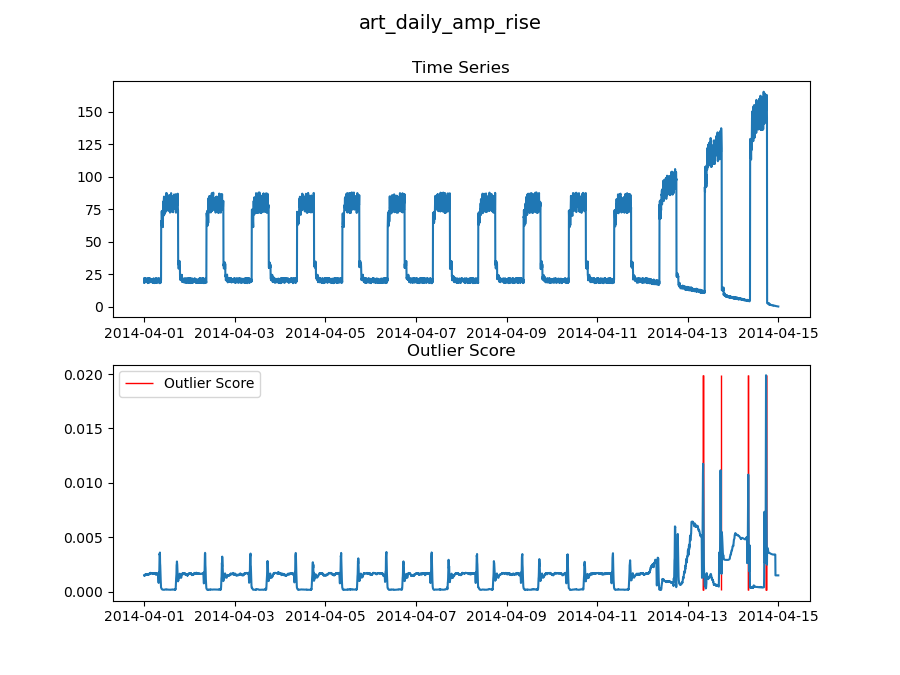
\includegraphics[width=0.5\textwidth]{fig/resultsIsoMap/art_daily_amp_rise}}
	\subfloat[Caption for sub-figure1]{
		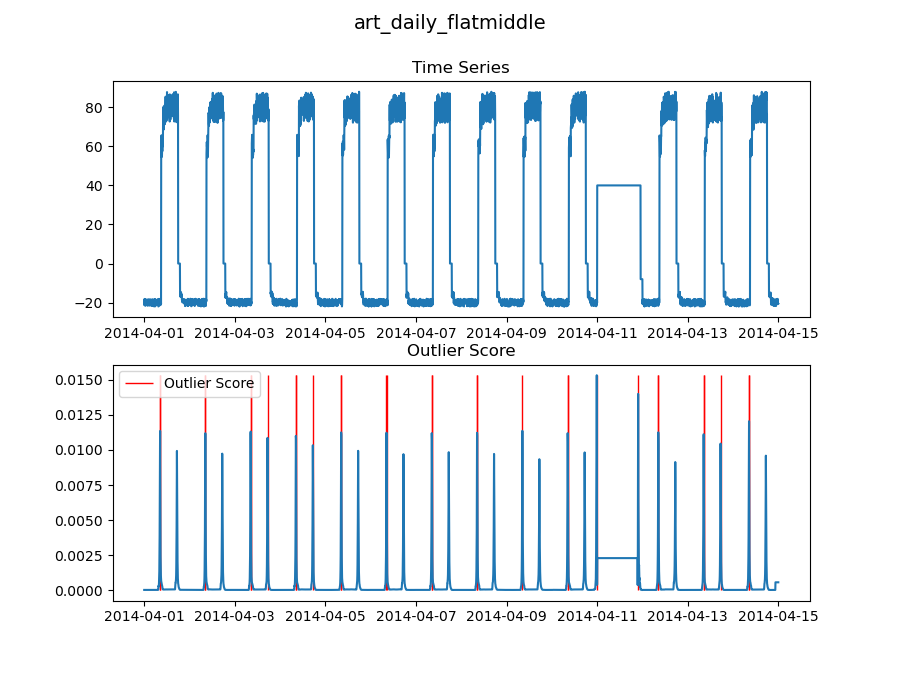
\includegraphics[width=0.5\textwidth]{fig/resultsIsoMap/art_daily_flatmiddle}}
	\qquad
	\subfloat[Caption for sub-figure1]{
		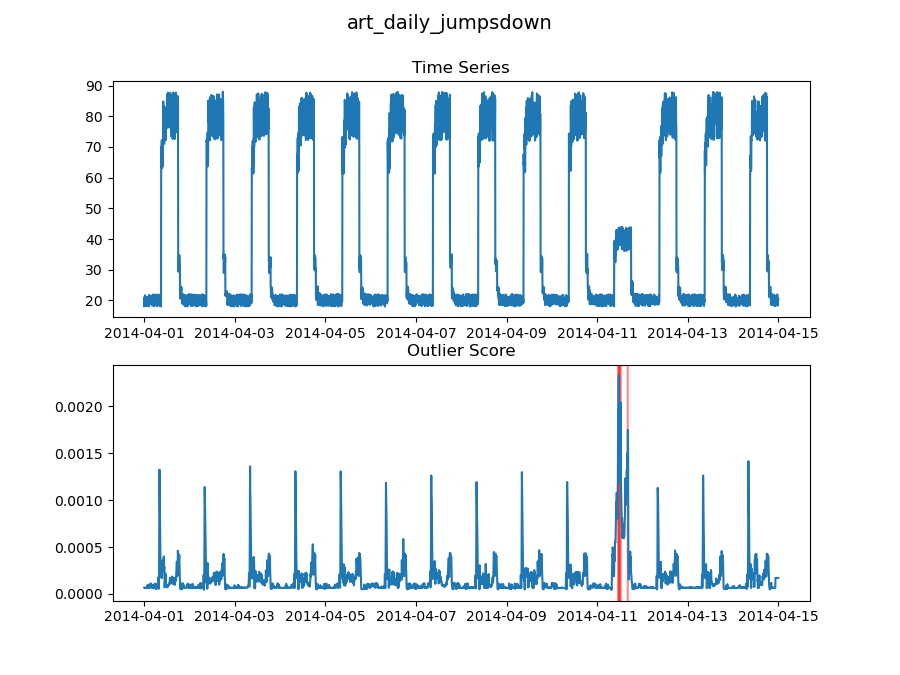
\includegraphics[width=0.5\textwidth]{fig/resultsIsoMap/art_daily_jumpsdown}}
	\subfloat[Caption for sub-figure1]{
		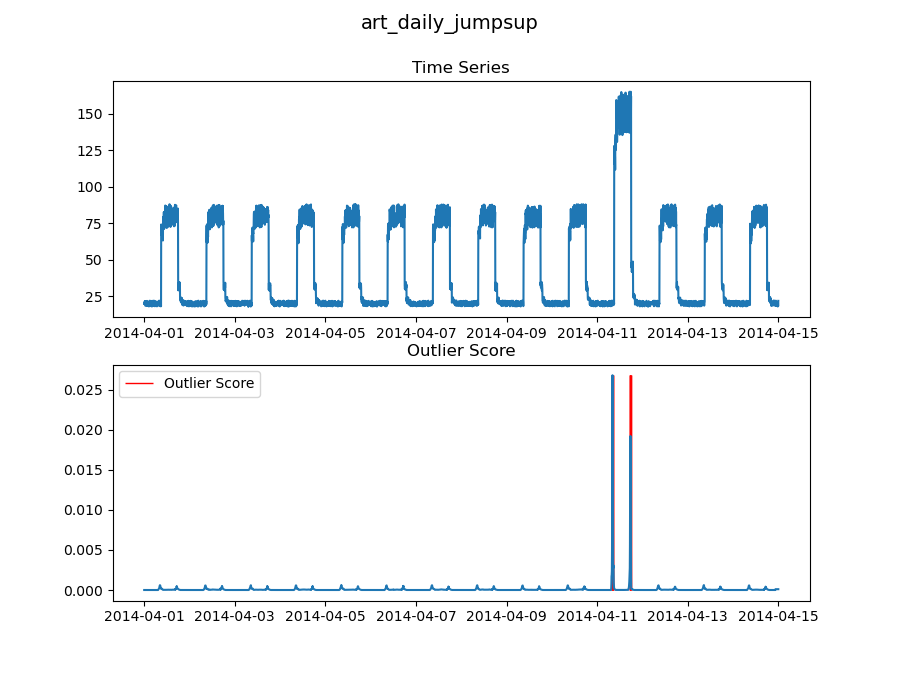
\includegraphics[width=0.5\textwidth]{fig/resultsIsoMap/art_daily_jumpsup}}
	\qquad
	\subfloat[Caption for sub-figure1]{
		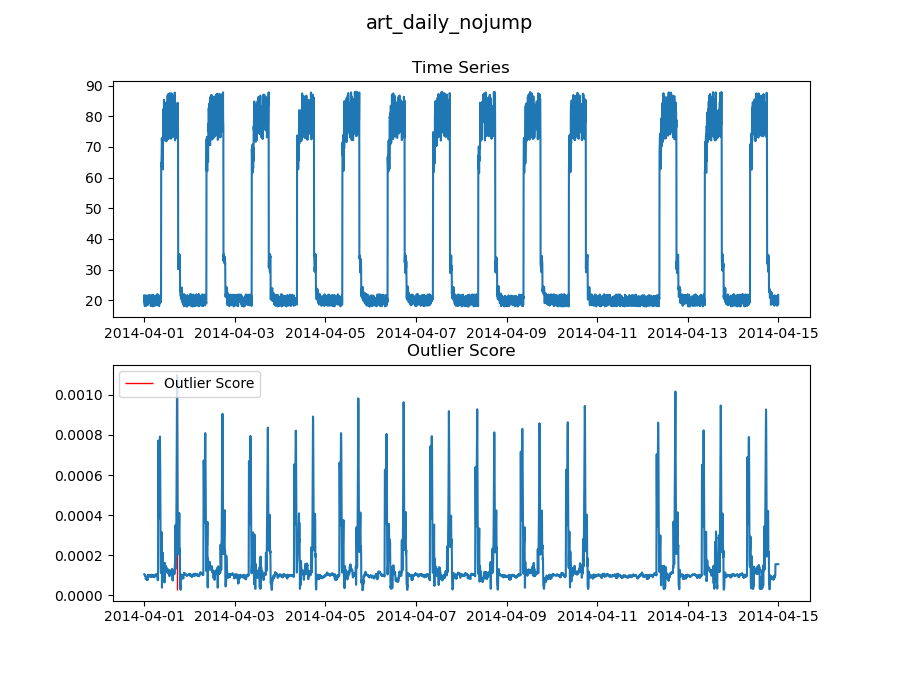
\includegraphics[width=0.5\textwidth]{fig/resultsIsoMap/art_daily_nojump}}
	\label{img:isomappictures2}
\end{figure}
\workTodo{In einigen Bilden fehlt die Legende. Vielleicht noch ein Paar bessere Ergebnisse zu erziehlen}





\newpage
\chapter{Perculation}
\section{Sliding Window}
\begin{figure}
	\centering
	\subfloat[Caption for sub-figure1]{
		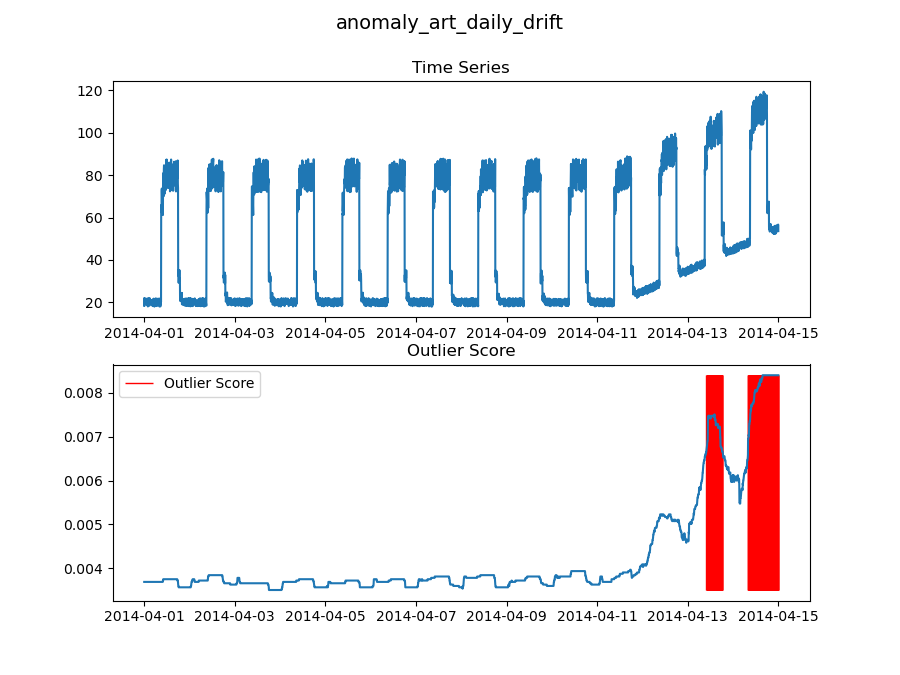
\includegraphics[width=0.5\textwidth]{fig/resultsPercolation/anomaly_art_daily_drift}}
	\subfloat[Caption for sub-figure1]{
		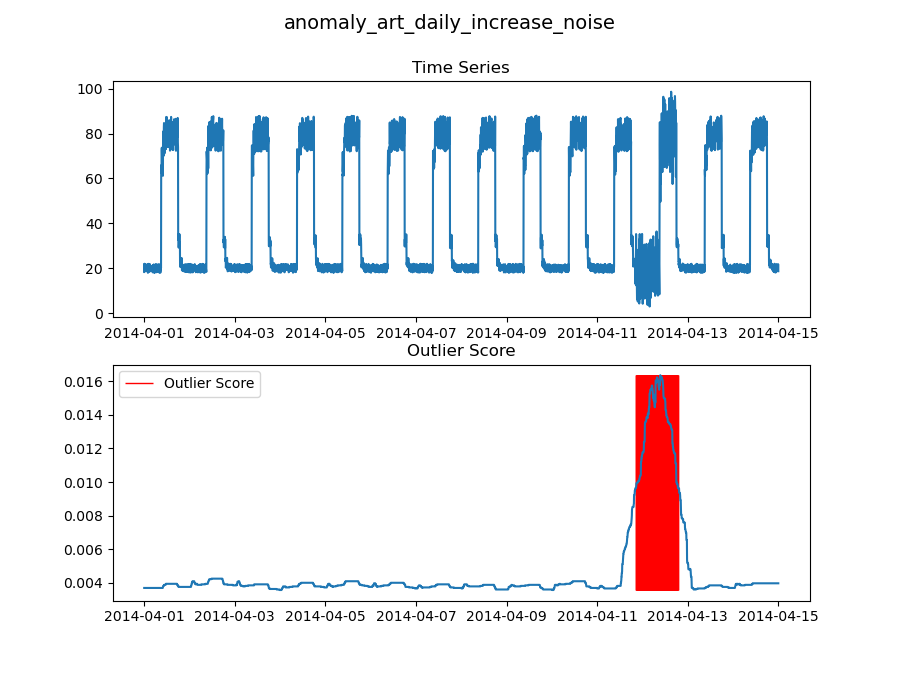
\includegraphics[width=0.5\textwidth]{fig/resultsPercolation/anomaly_art_daily_increase_noise}}
	\qquad
	\subfloat[Caption for sub-figure1]{
		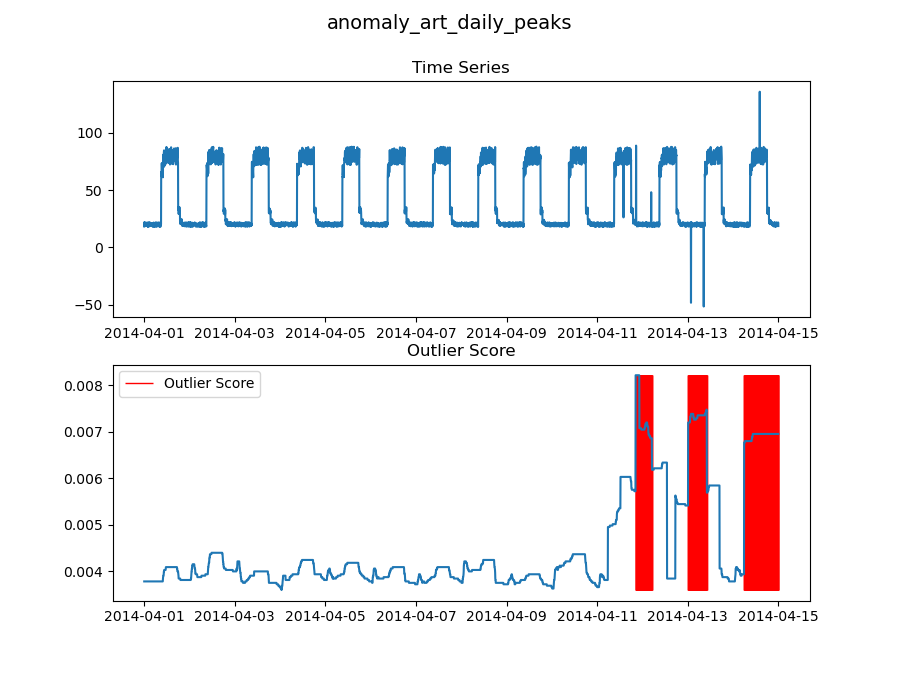
\includegraphics[width=0.5\textwidth]{fig/resultsPercolation/anomaly_art_daily_peaks}}
	\subfloat[Caption for sub-figure1]{
		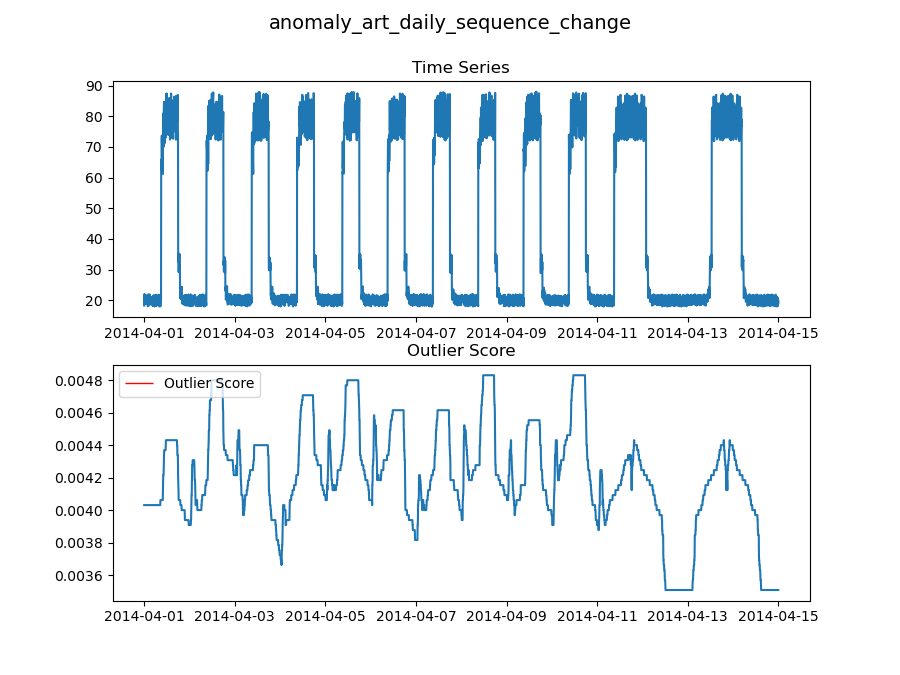
\includegraphics[width=0.5\textwidth]{fig/resultsPercolation/anomaly_art_daily_sequence_change}}
	\qquad
	\label{img:isomappictures1}
\end{figure}
\begin{figure}\ContinuedFloat
	\subfloat[Caption for sub-figure1]{
		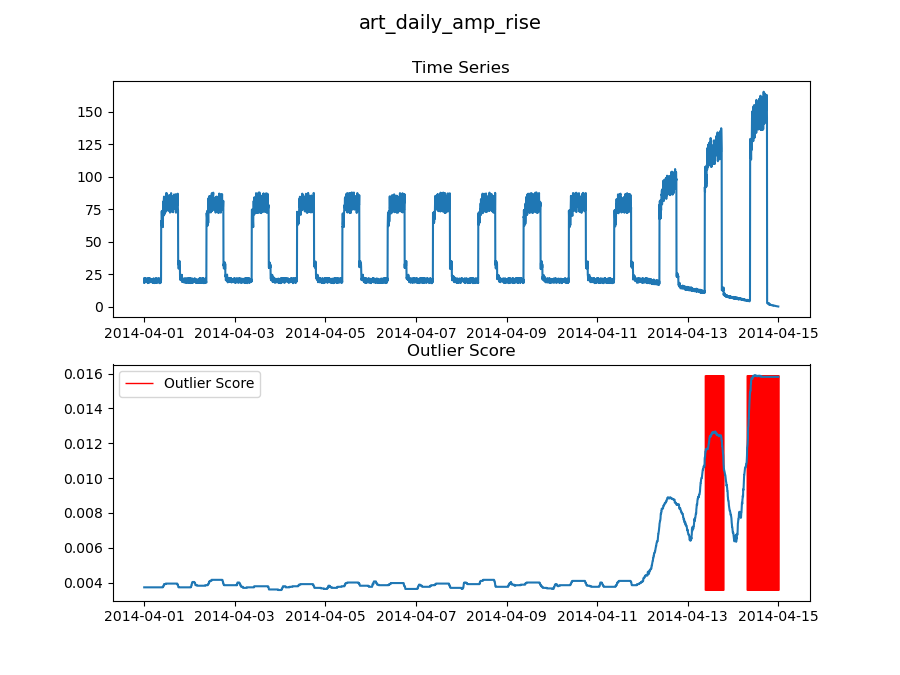
\includegraphics[width=0.5\textwidth]{fig/resultsPercolation/art_daily_amp_rise}}
	\subfloat[Caption for sub-figure1]{
		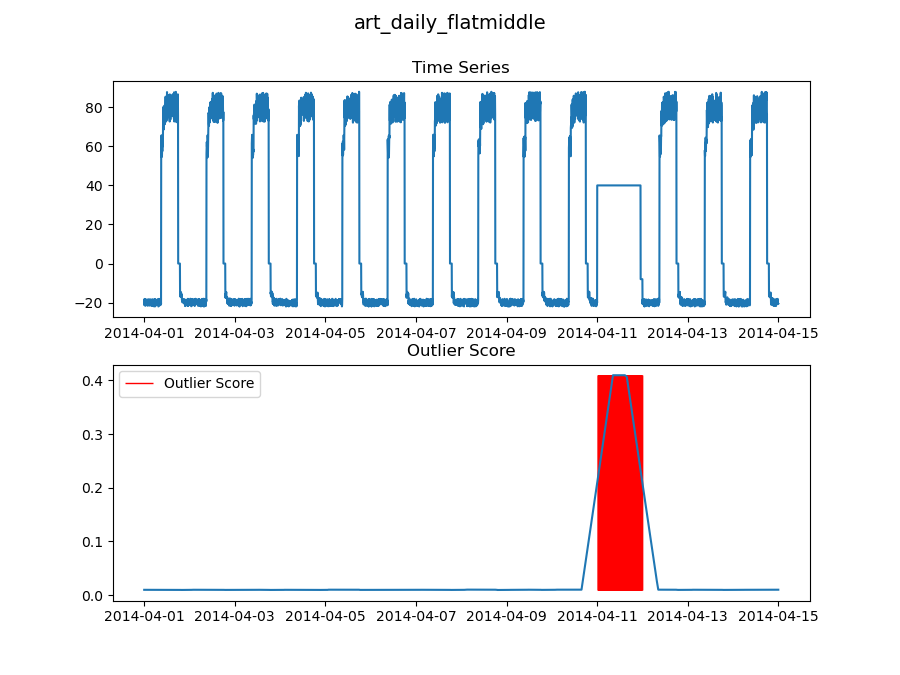
\includegraphics[width=0.5\textwidth]{fig/resultsPercolation/art_daily_flatmiddle}}
	\qquad
	\subfloat[Caption for sub-figure1]{
		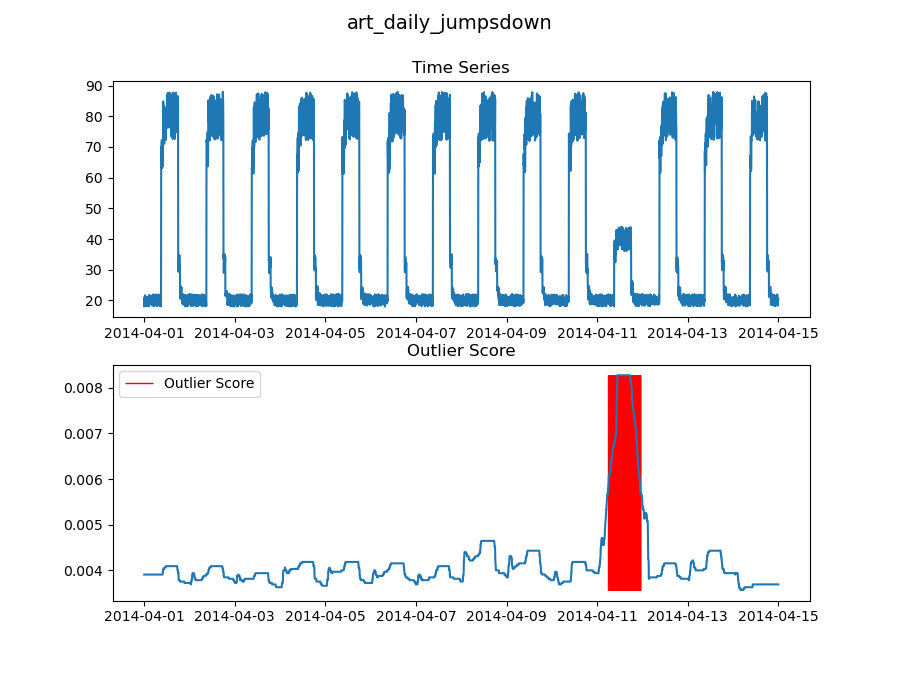
\includegraphics[width=0.5\textwidth]{fig/resultsPercolation/art_daily_jumpsdown}}
	\subfloat[Caption for sub-figure1]{
		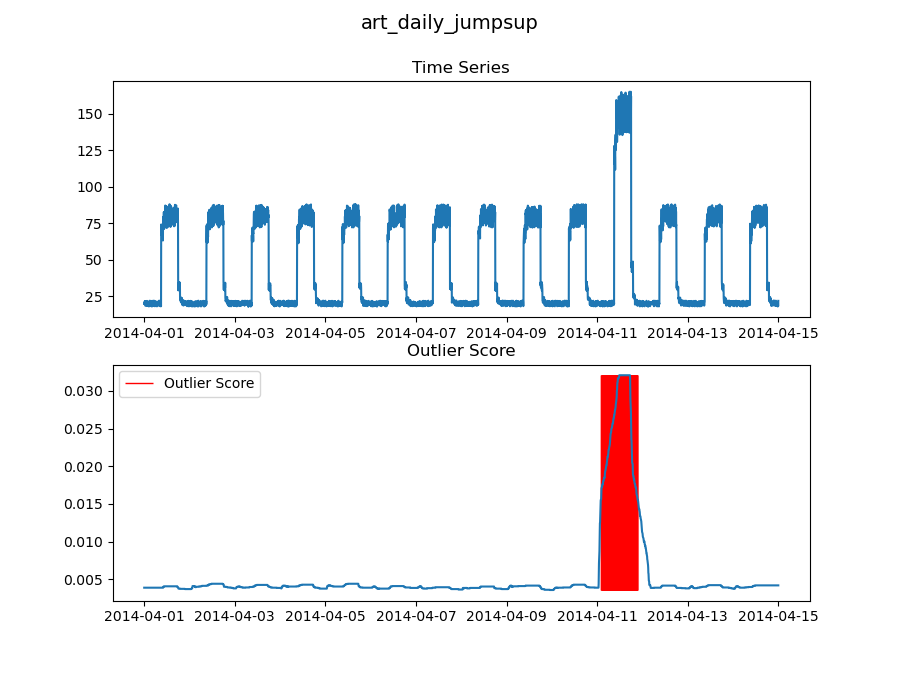
\includegraphics[width=0.5\textwidth]{fig/resultsPercolation/art_daily_jumpsup}}
	\qquad
	\subfloat[Caption for sub-figure1]{
		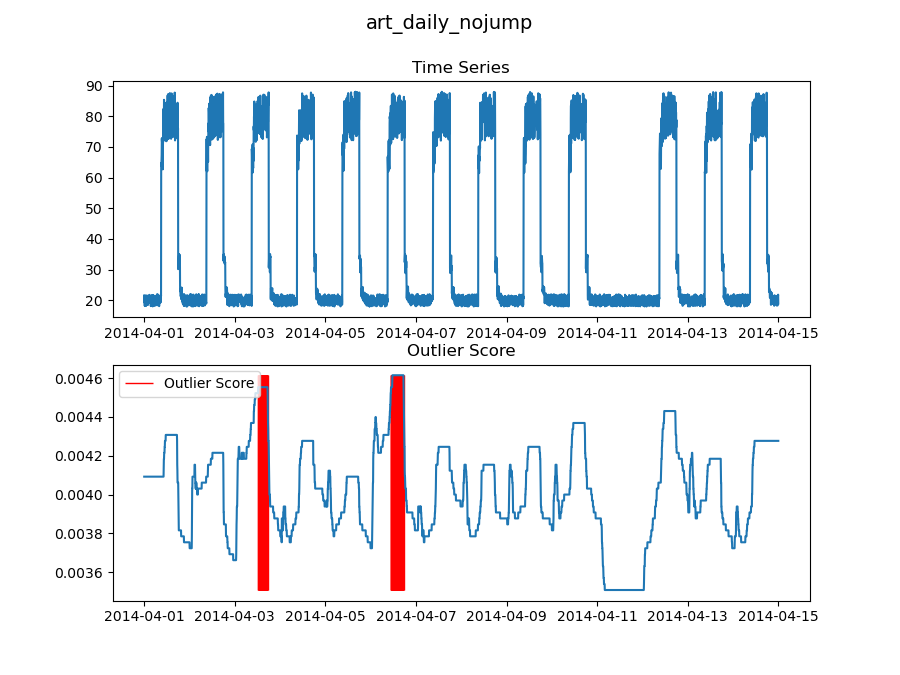
\includegraphics[width=0.5\textwidth]{fig/resultsPercolation/art_daily_nojump}}
	\label{img:isomappictures2}
\end{figure}


\newpage
\workTodo{Nim mir nicht sicher ob ich das ohne sliding window auch noch einfügen soll. Vielleicht kann ich oben ja einmal einen Vergleich mit sliding window und ohne sliding window rein machen}
